% Chapter Template

\chapter{Gated Recurrent Unit} % Main chapter title

\label{Chapter5} % Change X to a consecutive number; for referencing this chapter elsewhere, use \ref{ChapterX}

%----------------------------------------------------------------------------------------
%	SECTION 1
%----------------------------------------------------------------------------------------

\section{Understanding GRUs}

Gated recurrent units (GRUs) are a gating mechanism in recurrent neural networks, introduced in 2014 by Kyunghyun Cho et al \citation{Reference5}.

The GRU is like a LSTM with a forget gate but has fewer parameters than LSTM, as it lacks an output gate.

An scheme of a GRU architecture is described in figure \ref{fig:gru}.

\begin{figure}[H]
\begin{center}
  \makebox[\textwidth]{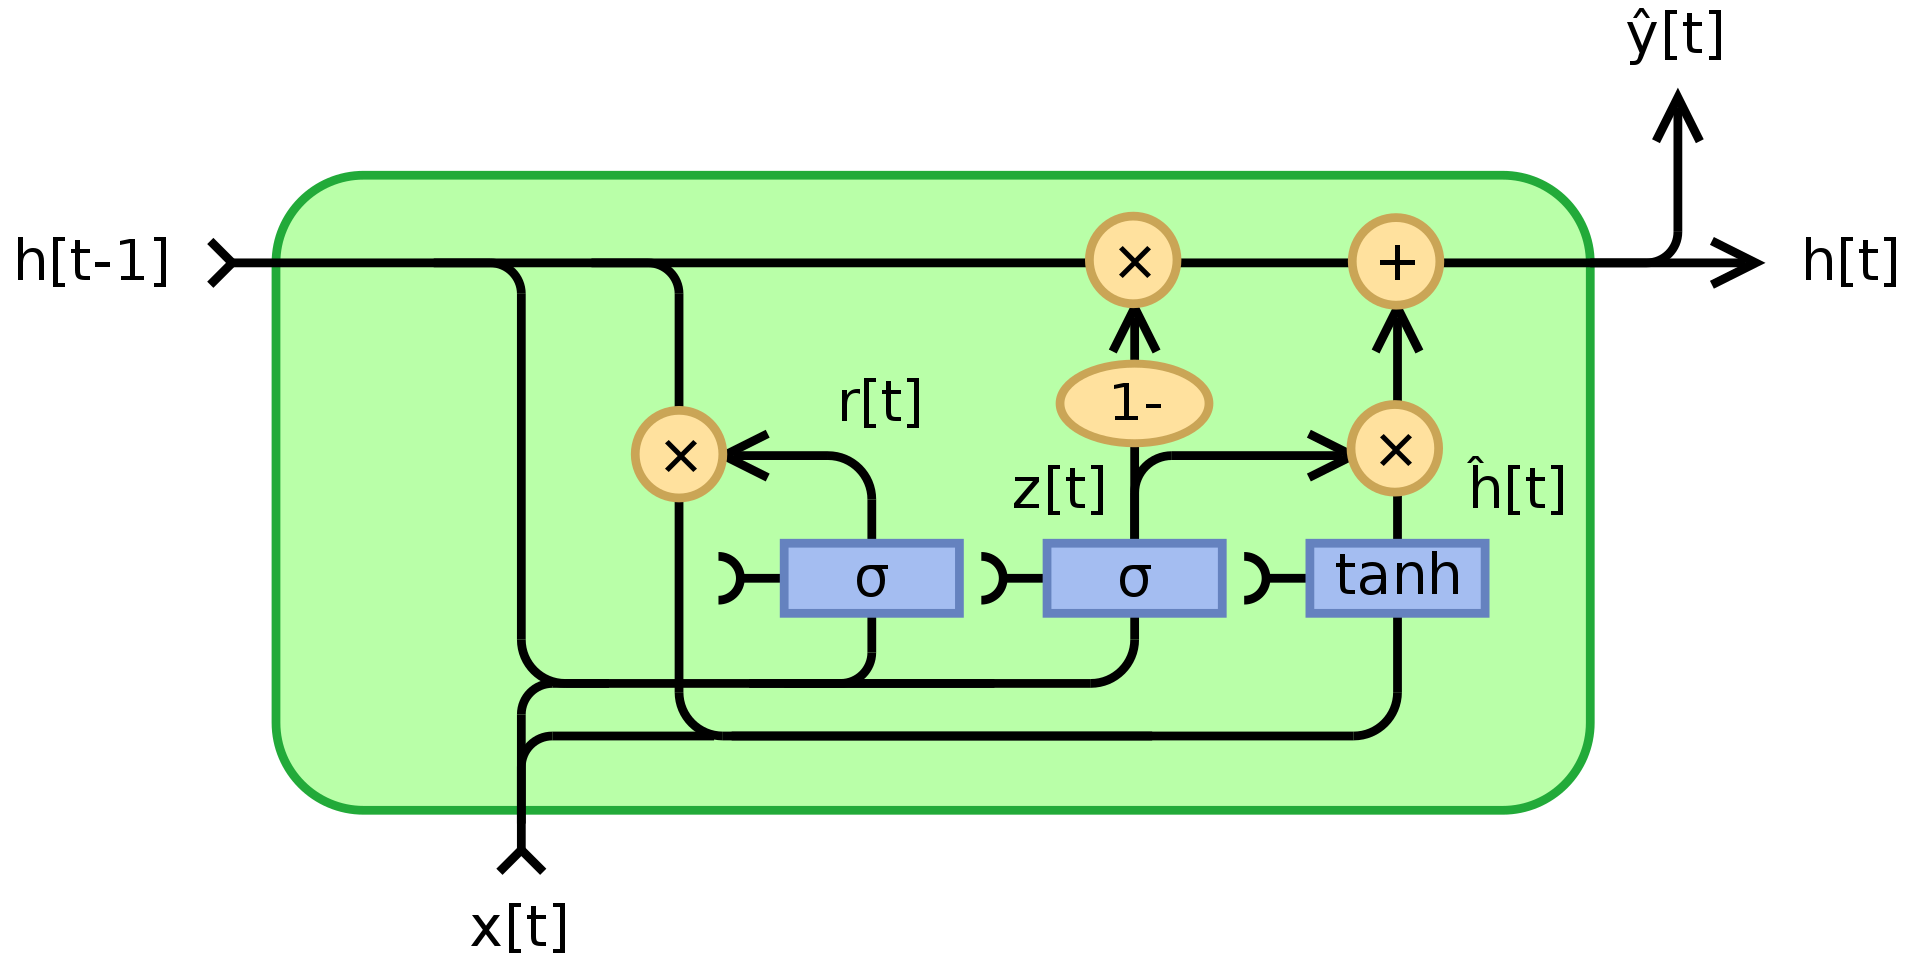
\includegraphics[width=\textwidth]{Figures/GRU}}
\end{center}
\decoRule
\caption[GRU architecture]{GRU architecture.}
\label{fig:gru}
\end{figure}

\section{Binary Classification}

The next sections describe the methodology applied to solve the binary classification problem using GRUs.

\subsection{Data Generation}

Before the ingestion of the data into the GRU model, it has to be adapted to the architecture of the network.

Being \textit{samples} the total number of data, \textit{timesteps} the amount of rows to be ingested for each aircraft and \textit{features} the number of sensor data the input of the GRU layer is defined by a tensor of shape:

\begin{verbatim}
    (samples, timesteps, features)
\end{verbatim}

The time steps used in this approach will be 50, which means that for each aircraft batches of 50 time steps will be taken.
Grouping the data this way, the total amount of input data will be 15631 matrices of (50, 25) shape.
As an example, for aircraft with id=1 the batches will be distributed this way:

\begin{verbatim}
    (0, 50)     -> from row 0 to row 50
    (1, 51)     -> from row 1 to row 51
    (2, 52)     -> from row 2 to row 52
    ...
    (111, 192)  -> from row 111 to row 192
\end{verbatim}

After the pre-processing, the input tensor will have the shape:

\begin{verbatim}
    (15631, 50, 25)
\end{verbatim}

To generate the labels, the values of the column \textit{label 1}, which was generated on the data preparation (see chapter \ref{Chapter3}), must be grouped by aircraft indicating if the engine failed within \textit{w1} cycles.

The result label tensor has the shape:

\begin{verbatim}
    (15631, 1)
\end{verbatim}

%-----------------------------------
%	SUBSECTION 2
%-----------------------------------

\subsection{Model definition}

This model is based on the previous one that focuses on the use of LSTM layers.
This time the same architecture, loss and activation functions are used but all the LSTM layers are switched by GRU layers.

Instead of adding Dropout layers, the dropout field provided by the Keras API implementation of the GRU layers is used.

The diagram for the neural network is described in figure \ref{fig:binary-gru-model}

\begin{figure}[H]
\centering
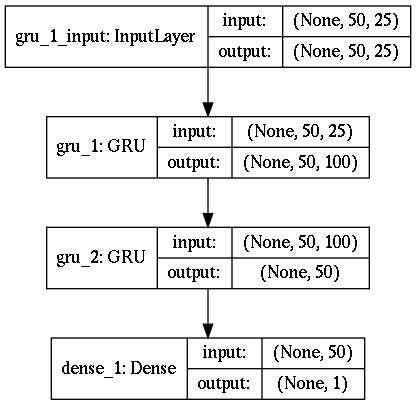
\includegraphics[scale=0.5]{Figures/binary-gru-model}
\decoRule
\caption[GRU Neural Network model for binary classification]{GRU Neural Network model for binary classification.}
\label{fig:binary-gru-model}
\end{figure}

\subsection{Training visualization}

As done in the previous model, the output of the second RNN layer has been visualized.
In this case the second GRU layer is the one selected.
The output of this layer is a tensor of size 50, which represents the hidden units of the GRU.
To extract the information contain by those celds, the \textit{Principal Component Analysis} (PCA) function has been chosen.

In figure \ref{fig:binary-gru-pca} you can see a graphical representation of this components.

As happened with the LSTM model, two separated clusters can be seen in the image.
This follows to the same conclusion, the data tends to split into two different options: the aircraft fails in a cycle or it doesn't.

\begin{figure}[H]
\centering
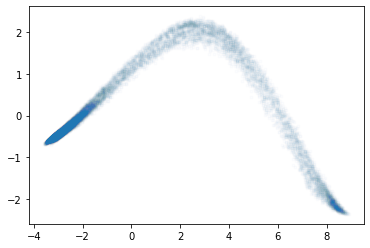
\includegraphics{Figures/gru-visualization}
\decoRule
\caption[PCA applied over GRU output]{PCA applied over GRU output.}
\label{fig:binary-gru-pca}
\end{figure}


\subsection{Results and model evaluation}

After the model is trained using batches of data of size 200. The validation split selected for the data is 5\%.

The evolution of the loss and accuracy during the model training can be seen in the figures \ref{fig:binary-gru-loss} and \ref{fig:binary-gru-acc}

The final accuracy obtained is 97\% so we can conclude that the network works very well for this task. To evaluate the results against the ground truth data a comparison graph has been generated. This graph can be seen in figure \ref{fig:binary-gru-results}.

\begin{figure}[H]
\begin{center}
  \makebox[\textwidth]{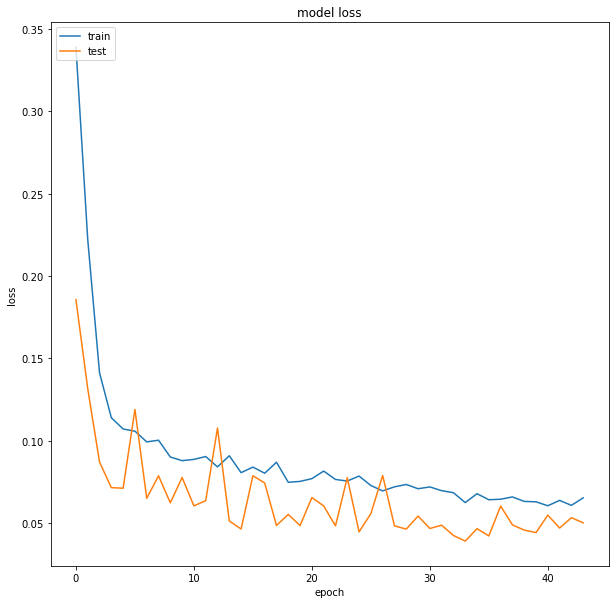
\includegraphics[width=\textwidth]{Figures/binary-gru-loss}}
\end{center}
\decoRule
\caption[GRU Binary Classification Model Loss]{GRU Binary Classification Model Loss.}
\label{fig:binary-gru-loss}\end{figure}

\begin{figure}[H]
\begin{center}
  \makebox[\textwidth]{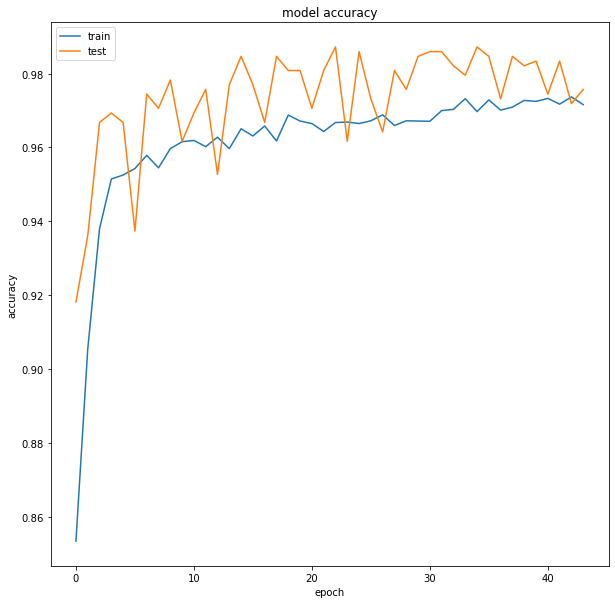
\includegraphics[width=\textwidth]{Figures/binary-gru-acc}}
\end{center}
\decoRule
\caption[GRU Binary Classification Model Accuracy]{GRU Binary Classification Model Accuracy.}
\label{fig:binary-gru-acc}
\end{figure}

\begin{figure}[H]
\begin{center}
  \makebox[\textwidth]{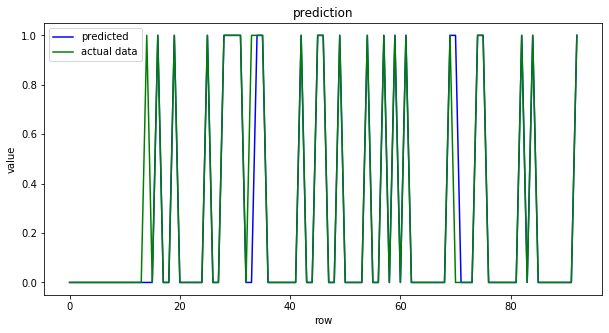
\includegraphics[width=\textwidth]{Figures/binary-gru-results}}
\end{center}
\decoRule
\caption[Result comparison between Binary GRU Model and Ground Truth data]{Result comparison between Binary GRU Model and Ground Truth data.}
\label{fig:binary-gru-results}
\end{figure}


\section{Regression Model}

The next sections describe the methodology applied to solve the regression problem using GRUs


\subsection{Data Generation}

Before the ingestion of the data into the GRU model, it has to be adapted to the architecture of the network.

Being \textit{samples} the total number of data, \textit{timesteps} the amount of rows to be ingested for each aircraft and \textit{features} the number of sensor data the input of the LSTM layer is defined by a tensor of shape:

\begin{verbatim}
    (samples, timesteps, features)
\end{verbatim}

The time steps used in this approach will be 50, which means that for each aircraft batches of 50 time steps will be taken.
Grouping the data this way, the total amount of input data will be 15631 matrices of (50, 25) shape.
As an example, for aircraft with id=1 the batches will be distributed this way:

\begin{verbatim}
    (0, 50)     -> from row 0 to row 50
    (1, 51)     -> from row 1 to row 51
    (2, 52)     -> from row 2 to row 52
    ...
    (111, 192)  -> from row 111 to row 192
\end{verbatim}

After the pre-processing, the input tensor will have the shape:

\begin{verbatim}
    (15631, 50, 25)
\end{verbatim}

For this type of regression model the labels are the values of the column \textit{RUL}, which was generated on the data preparation (see chapter \ref{Chapter3}).

The result label tensor has the shape:

\begin{verbatim}
    (15631, 1)
\end{verbatim}


\subsection{Model definition}

Like the binary one, this model has been created just replacing the LSTMs layers used in the previous chapter with GRU layers.
The rest of the components of the model remain the same.

It is interesting to notice that in order to make the model converge, specific Dropout layers has been used instead that the features provided by the GRU layer API.

The diagram for the neural network is described in figure \ref{fig:regression-gru-model}

\begin{figure}[H]
\centering
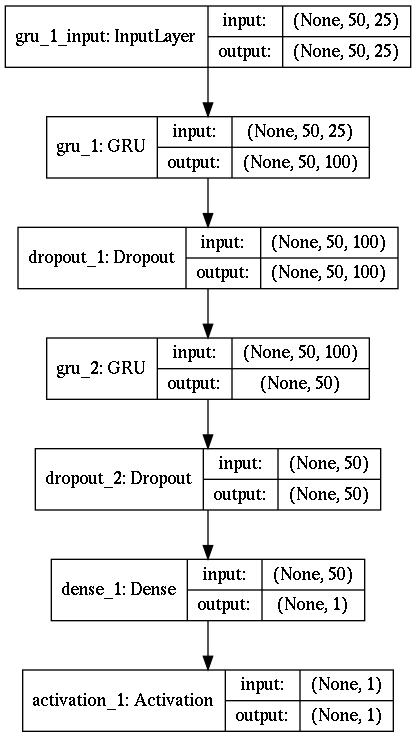
\includegraphics[scale=0.5]{Figures/regression-gru-model}
\decoRule
\caption[Neural Network for GRU regression model]{Neural Network for GRU regression model.}
\label{fig:regression-gru-model}
\end{figure}

\subsection{Results and model evaluation}

After the model is trained using batches of data of size 200.
The validation split selected for the data is 5\%.

The evolution of the loss and metrics during the model training can be seen in the figures \ref{fig:regression-gru-loss}, \ref{fig:regression-gru-r2} and \ref{fig:regression-gru-mae}

The final results obtained for \textit{MAE} and \textit{R-square} are 13.70 and 0.81 respectively.
To evaluate the results against the ground truth data a comparison graph has been generated. This graph can be seen in figure \ref{fig:regression-gru-results}.

\begin{figure}[H]
\begin{center}
  \makebox[\textwidth]{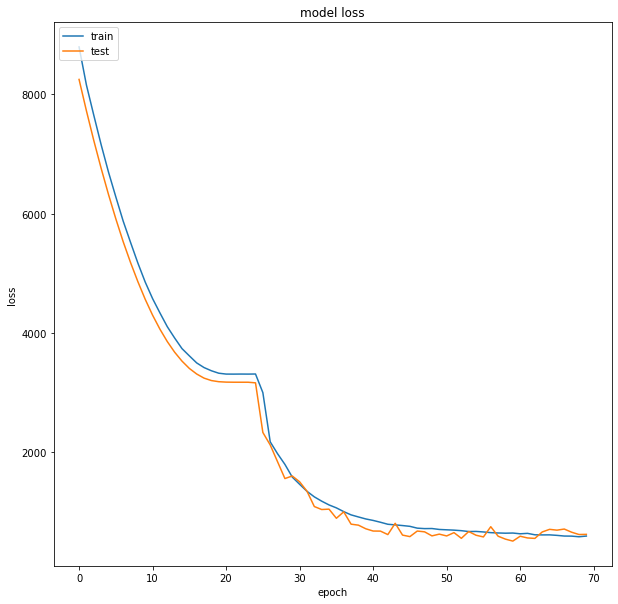
\includegraphics[width=\textwidth]{Figures/regression-gru-loss}}
\end{center}
\decoRule
\caption[GRU Regression Model Loss]{GRU Regression Model Loss.}
\label{fig:regression-gru-loss}\end{figure}

\begin{figure}[H]
\begin{center}
  \makebox[\textwidth]{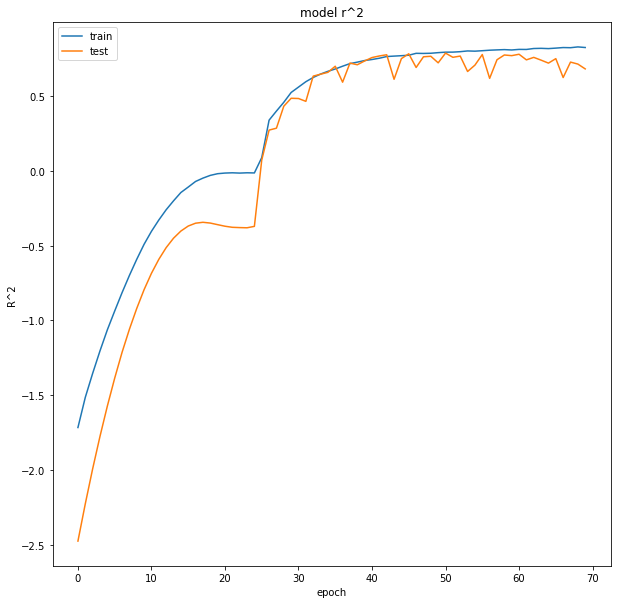
\includegraphics[width=\textwidth]{Figures/regression-gru-r2}}
\end{center}
\decoRule
\caption[GRU R2 model]{GRU R2 model.}
\label{fig:regression-gru-r2}
\end{figure}

\begin{figure}[H]
\begin{center}
  \makebox[\textwidth]{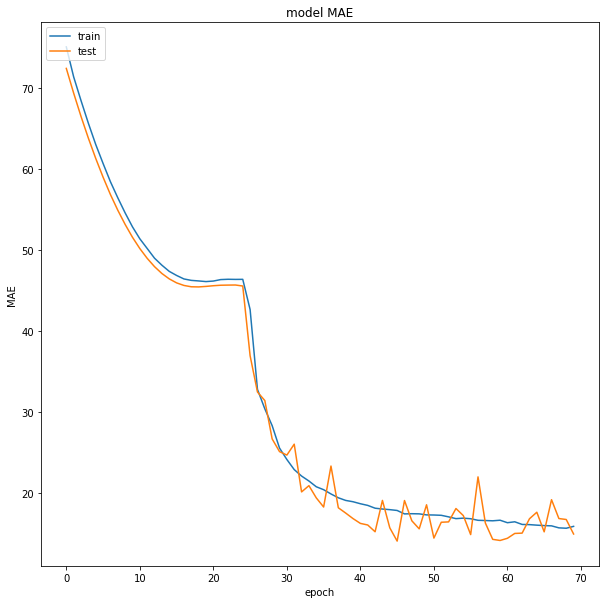
\includegraphics[width=\textwidth]{Figures/regression-gru-mae}}
\end{center}
\decoRule
\caption[GRU MAE model]{GRU MAE model.}
\label{fig:regression-gru-mae}
\end{figure}

\begin{figure}[H]
\begin{center}
  \makebox[\textwidth]{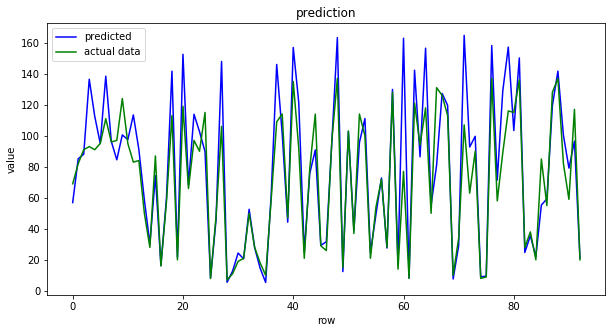
\includegraphics[width=\textwidth]{Figures/regression-gru-results}}
\end{center}
\decoRule
\caption[Result comparison between Regression GRU Model and Ground Truth data]{Result comparison between Regression GRU Model and Ground Truth data.}
\label{fig:regression-gru-results}
\end{figure}
